\section{2D Spoked Runners}

Extended from the vertical hopper, this model is aimed to use for analysis of coupled dynamics of the spoked runner, which has following assumptions

\begin{itemize}
\item massless leg 
\end{itemize}


\subsection{SLIP model with a locked flywheel}
Compared to \cite{Shen2016}, this is a model which is genearlized so that the rotation in the flight phase can also be considered.
\begin{figure}[h]
\centering

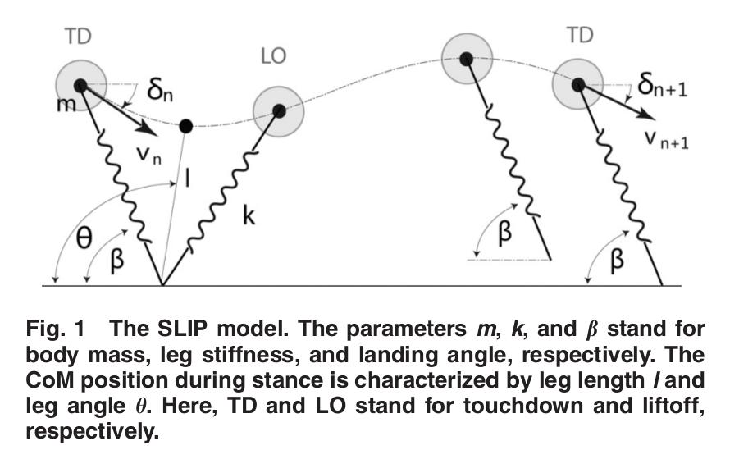
\includegraphics[scale=0.75]{SLIPmodel.pdf}
\caption{The schematic of a SLIP model }
\label{fig.SLIPmodel}
\end{figure}

\subsubsection{System Kinematics}
As indicated in Fig \ref{fig.SLIPmodel}, the position of the body (mass) is
\begin{align*}
x &= -lcos\theta\\
z &= lsin\theta\\
\end{align*}
and the velocity
\begin{align*}
\dot x &= -\dot lcos\theta +lsin\theta\dot \theta\\
\dot z &= \dot lsin\theta + lcos\theta \dot{\theta}\\
\end{align*}





\subsubsection{Lagrangian Mechanics}
Wit the velocity of the mass, the Lagrangian $L$ can be expressed as:
\begin{align*}
L &= T-V = \frac{1}{2}m(\dot x^2+\dot y^2) + \frac{1}{2}I\dot\theta^2 - V_{spring} - V_{gravity}\\
 &= \frac{1}{2}m(\dot l^2 + l^2\dot \theta^2 )+ \frac{1}{2}I\dot\theta^2 - \frac{1}{2}k(l-l_0)^2-mg(lsin\theta)
\end{align*}


\noindent
where $I = mr_g^2$. Take $l$, $\theta$ as the generalized coordinate, the equation of motions are:\\
\noindent
\textbf {Stance Dynamics}
\begin{align*}
m\ddot{l} - ml^2\dot{\theta}^2 + k(l-l_0) &= -mgsin\theta\\
2ml\dot l \dot{\theta} + m(l^2+r_g^2)\ddot{\theta} +   &= -mglcos\theta
\end{align*}
\noindent
\textbf {Flight Dynamics}
\begin{align*}
\ddot y &= -g\\
\ddot \theta &= 0\\
\text{LO: } l &= l_0\\
\text{TD: } y &= l_0sin\beta\\
\text{(Spoked TD: } \theta &= \beta + \frac{2\pi}{d}\text{)}
\end{align*}
where $\beta$ is the touch down angle, $d$ is the number of the legs the spoked runner has.\\
\textbf{Note:} when $I = 0$, the system is equivalent to the transitional SLIP model as described in  \cite{Shen2016}.



\subsubsection{EOM of SLIP model with a locked fly wheel}
This is an extended model which is used for the stability analysis of the 2D spoked (or reciprocating) runner.\\
\textbf{Note:} In the flight phase there will be the inertia at COM (the two masses connected via the link with length $r_c$), therefore no flywheel is required for the rotation EOM.


\subsection{SLIP with a PEndulum Runner (SLIPPER)}
\begin{figure}[h]
\centering

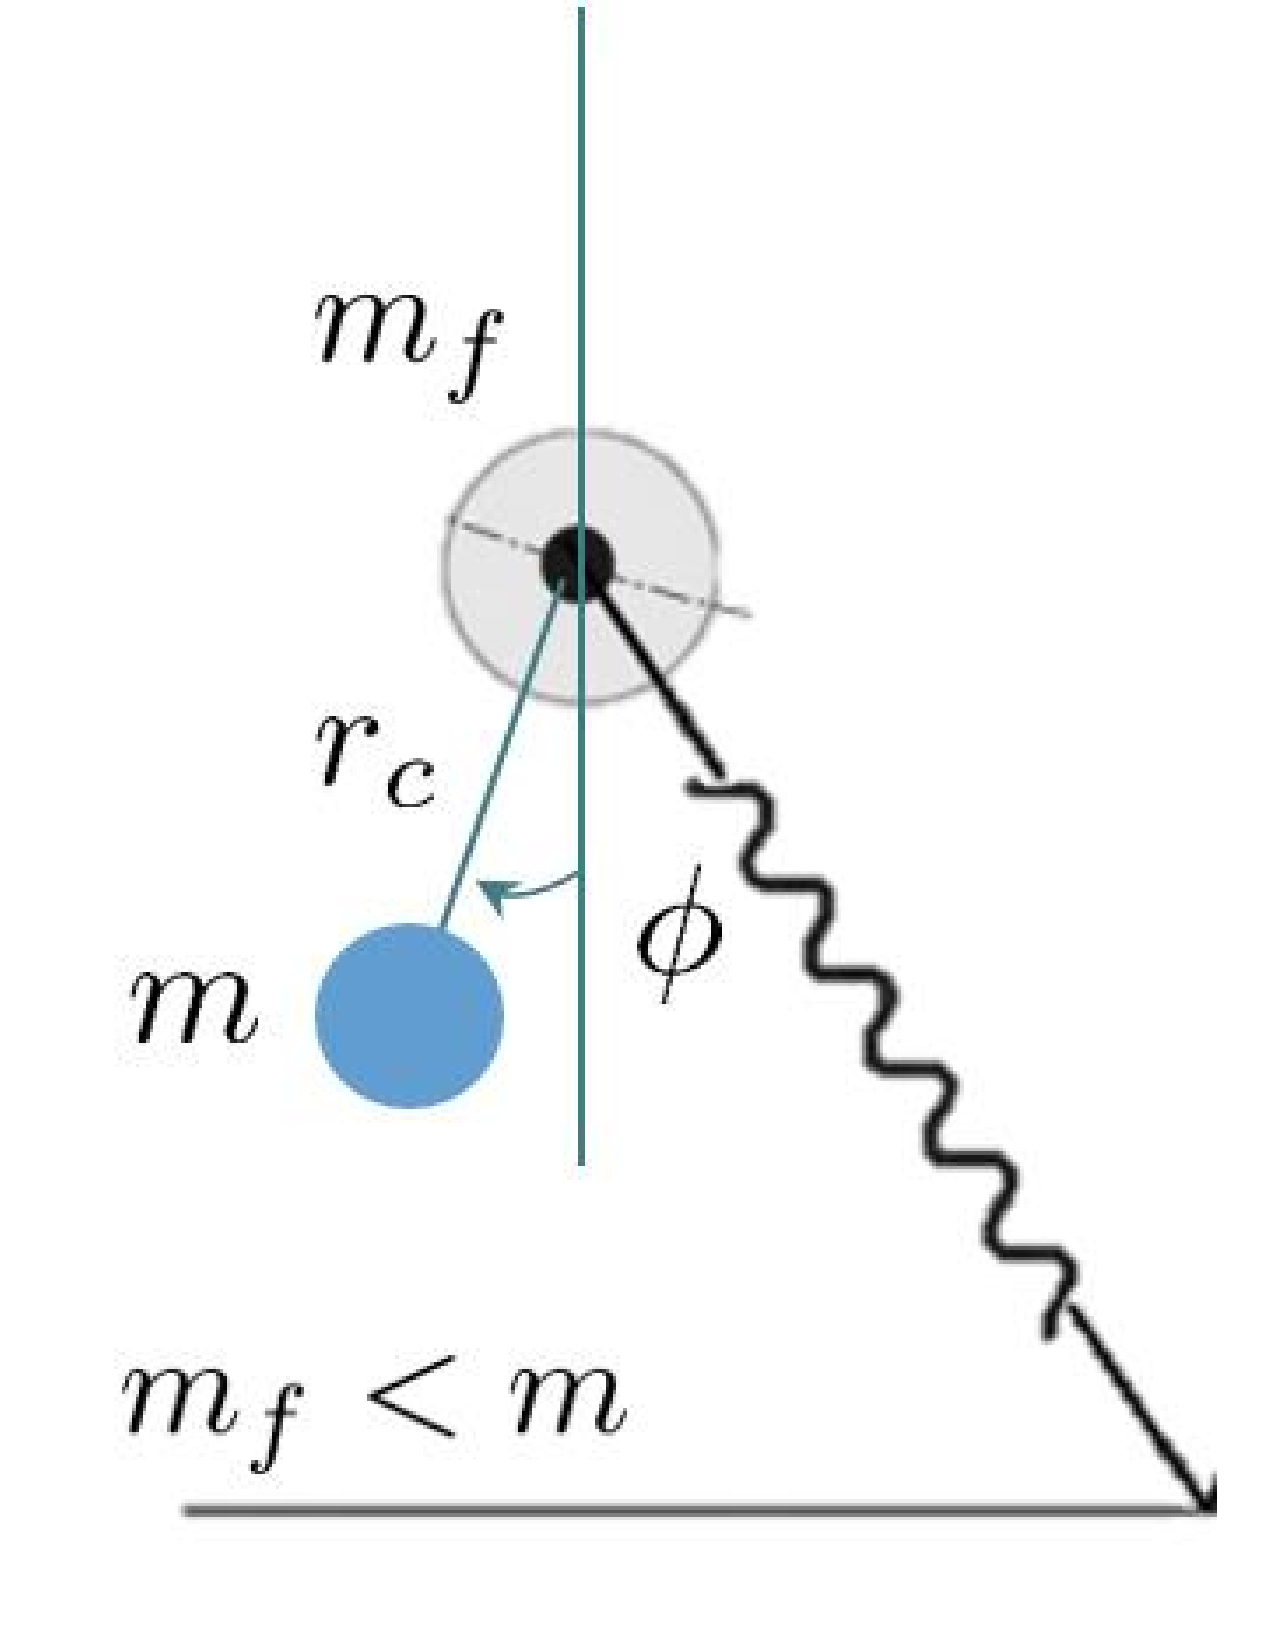
\includegraphics[scale=0.15]{SLIPPER.pdf}
\caption{The schematic of a SLIPPER}
\label{fig.SLIPPER}
\end{figure}

\subsubsection{System Kinematics}
As indicated in Fig \ref{fig.SLIPPER}, the position 
and the velocity of the frame $m_f$ are:
\begin{align*}
x_f &= -lcos\theta \\
z_f &= lsin\theta \\
	\dot x_f &= -\dot lcos\theta + lsin\theta\dot \theta \\
\dot z_f &= \dot lsin\theta + lcos\theta \dot{\theta}
\end{align*}
The position 
and the velocity of the body $m_b$ are:
\begin{align*}
x_b &= -lcos\theta - r_csin(\phi)\\
z_b &= lsin\theta - r_ccos(\phi)\\
\dot x_b &= -\dot lcos\theta +lsin\theta\dot \theta -  r_ccos(\phi)(\dot\phi)\\
\dot z_b &= \dot lsin\theta + lcos\theta \dot{\theta} + r_csin(\phi)(\dot\phi)\
\end{align*}


\subsubsection{System Dynamics}


Derived by the Lagrangian mechanics, the equation of motion of the stance phase in matrix form:

\begin{align}
\label{eq:EOM_SLIPP}
\nonumber \ddot X &= 
\begin{bmatrix}
\ddot l  \\
\ddot \theta\\
\ddot \phi  \\
\end{bmatrix} \\ &= M^{-1} b\\
LO: l&=0\\
\end{align}
where $M$ is the inertia matrix, $b$ is the nonlinear terms including velocity product and gravity force. For the symbolic expression please check the project Repo in stash:
\href{https://stash.ihmc.us/projects/ICSL/repos/fast-runner-analysis}{https://stash.ihmc.us/projects/ICSL/repos/fast-runner-analysis}\\

\subsubsection{System Dynamics with torque applied to the pendulum}
\begin{figure}[h]
	\centering
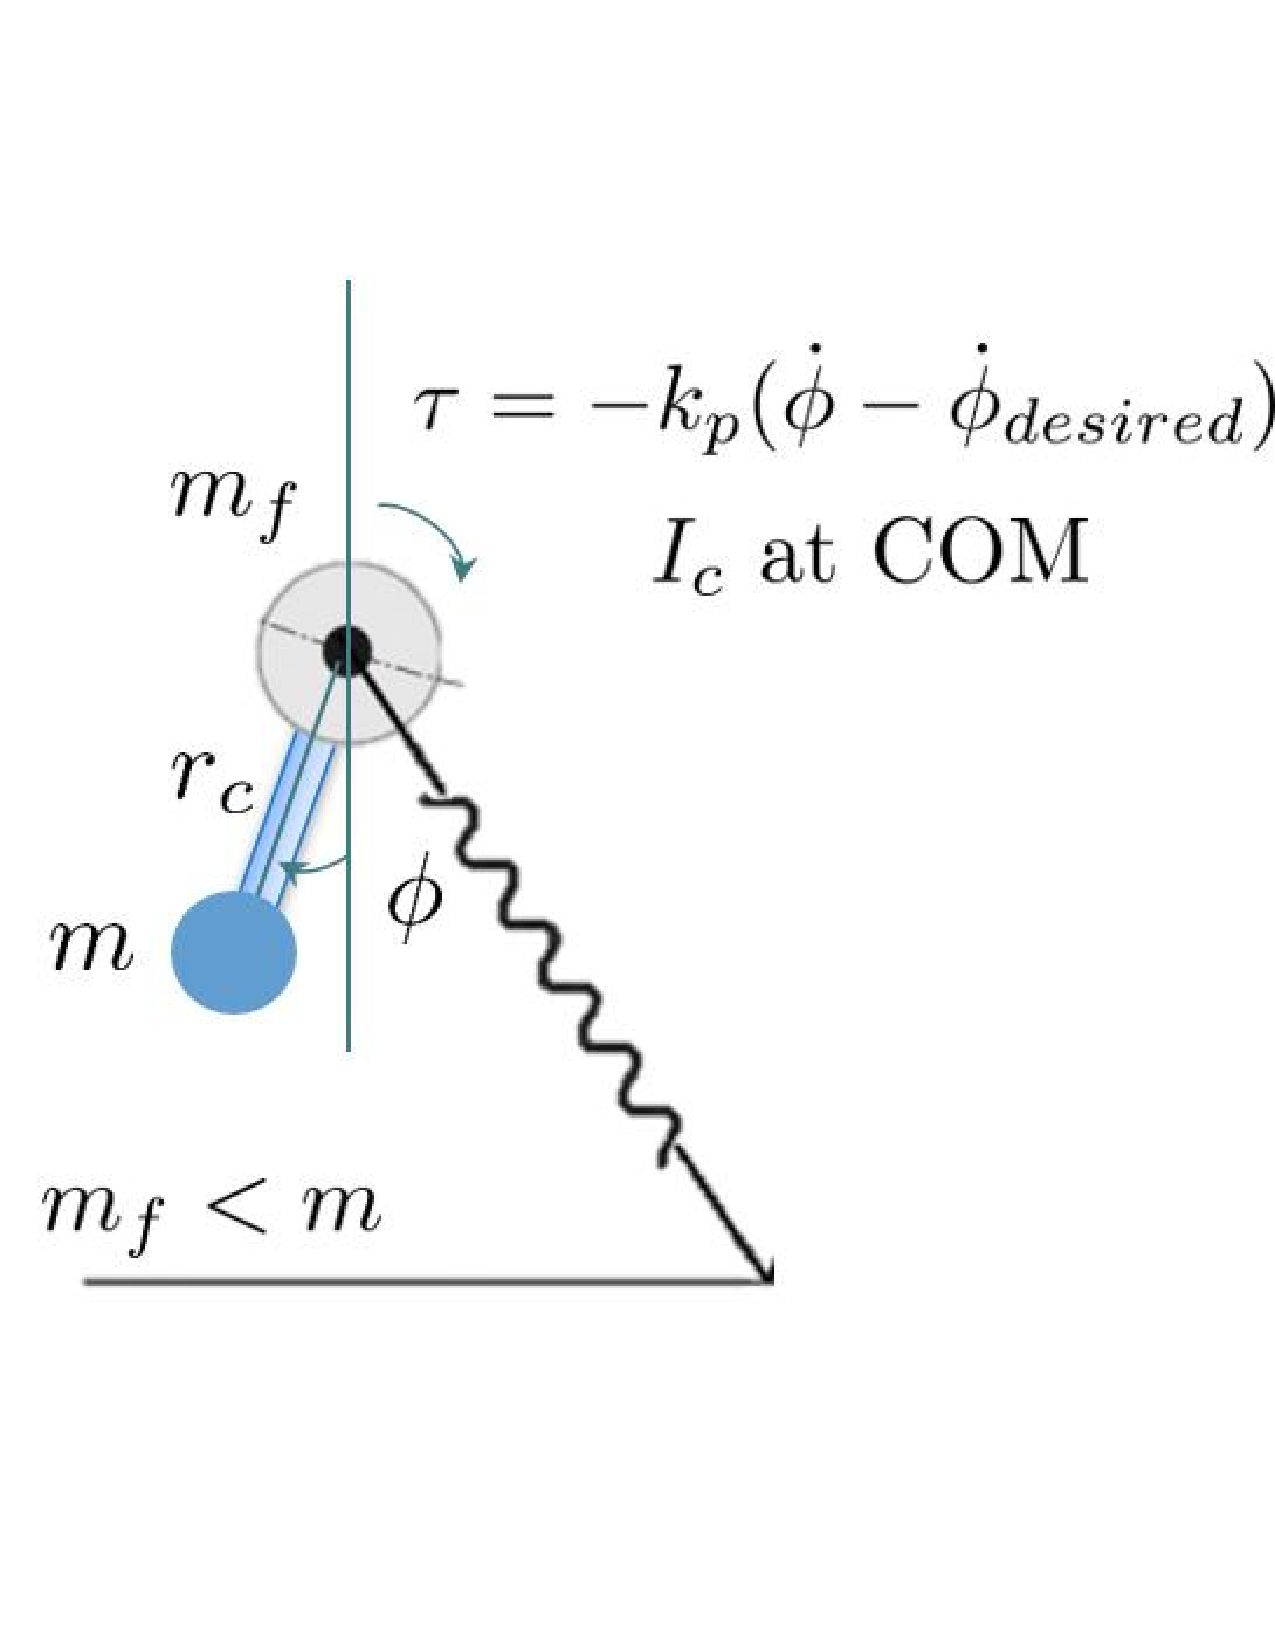
\includegraphics[scale=0.2]{SLIPPER_Inertia_Control.pdf}
\caption{The schematic of a SLIPPER with inertia and COM and torque control}
\label{fig.SLIPPER_Inertia_Control}
\end{figure}
In the last implementation during this project, an inertia $I_c$ at COM and a torque $\tau$ is added to the SLIPPER model.  Defining the relative angle between the leg and the pendulum as $(\phi-\theta+\pi/2)$ and a torque $\tau$ can be exerted between the leg and the pendulum, then by virtual work the torque can be added to the EOMs as follows:

\begin{align}
\label{eq:EOM_SLIPPCtrl}
\nonumber \ddot X &= 
\begin{bmatrix}
\ddot l  \\
\ddot \theta\\
\ddot \phi  \\
\end{bmatrix} \\ &= M^{-1} b +
\begin{bmatrix}
 0  \\
 -\tau\\
 \tau  \\
\end{bmatrix}\\
LO: l&=0\\
\end{align}
where $\tau = -k_p(\dot\phi-\dot{\phi}_{desired})$. Note: after discussing with Jerry in the last meeting, he suggested that the I should try to implement the p control for the relative angular velocity between the pendulum and the leg (i.e. $\dot \phi-\dot \theta$) instead of the absolute angular velocity $\dot\phi$, because the later will need a IMU. Unfortunately I did not have enough time to try it, so I made a note here.\\ 

\noindent Equation of motion in flight phase will be the same since the torque can only be applied in the stance phase.

\subsection{Dimension analysis and Physical meanings of parameters}
Followed the work from Shen's analysis of SLIP model \cite{Shen2016}, the dimension analysis is applied to the SLIPPER as well. The advantage of dimension analysis includes:

\begin{itemize}
	\item Make the model can be scaled to any geometry or weight.
	\item Fewer free variables in the trajectory optimization using single shooting method.
	\item Downside: harder to understand (for audience), and the math can easily go wrong if the dimension analysis does not perform properly.
\end{itemize}

\noindent Key parameters of the SLIP-based model in the stability analysis:

\begin{itemize}
	\item $\beta$: touchdown angle (i.e. foot placement.)
	\item $\tilde g = \frac{gl_0}{v_0^2} \rightarrow$ Smaller $\tilde g$, higher running speed! (Also in most of the presentation I made, I usually assume leg initial length $l_0=1$. Also, it kind of making sense that if the running speed goes higher, the effect from the gravity will become smaller (so in the extremely fast speed, it will be almost like it is flying.)
	\item $\tilde k = \frac{kl_0^2}{mv_0^2} = 1/(I^2_{fast-running}\tilde \beta^2)$, where $\tilde\beta = \frac{\pi/2-\beta}{\pi/2} \rightarrow$ lower $\tilde{k}$, larger fast running index $I_{fast-running}$!. Please note in the fast runner document from IHMC, the touchdown angle definition is different from the main reference \cite{Shen2016} used in the stability analysis.
\end{itemize}

\noindent Note about mass scaling for SLIPPER: In the dynamics used in MATLAB I scale the mass by the body mass $m$, so the total weight of SLIPPER becomes $1+\tilde{m_f}$. To make a fair comparison to SLIP model, in the plotting function I rescaled the SLIPPER data again such that its total weight will be $1$ in that case.


\subsection{Optimization formulation for single shooting trajectory optimization}

\noindent \textbf{Optimization for the SLIP model:}\\

\begin{enumerate}
	\item For a given $\beta$, $\tilde g$, and $\tilde k$, and initial guess, solve the following optimization:
	\begin{equation*}
	\begin{aligned}
	& \underset{\delta^*=\delta_0}{\text{min}}
	& & f(\delta_0)=(\delta_0 -\delta_1)^2 + (\tilde v_0 -\tilde v_1)^2 \\
	\end{aligned}
	\end{equation*}
	where $f(\delta_0)$ is the output from oneStepSimulationSLIP.m with the option 'parms.mode = 'fixedPointOpt''.	
	\item Then, accept the solution if
	$f(\delta^*)<1e-6$ and $0<\delta^*<\pi/2$.
	\item  Next, Check the stability of fixed points:
	abs(eigen values) of $M$, 
	where $M = \frac{\partial f(x)}{\partial x}$, and $\epsilon = 1e-4$.	
\end{enumerate}
 


\noindent \textbf{Optimization for the SLIPPER model with inertia and control:}\\

\begin{enumerate}
	\item For a given $\delta$, $\beta$, $\tilde g$, and $\tilde k$, and initial guess, solve the following optimization:
	\begin{equation*}
	\begin{aligned}
	& \underset{x^*=[\phi^*,\dot\phi^*,\dot\phi_d^*]}{\text{min}}
	& & f(x)=3(\delta_0 -\delta_1)^2 + 3(\tilde v_0 -\tilde v_1)^2+(\phi_0 -\phi_1)^2+(\dot\phi_0 -\dot\phi_1)^2+0.01(\dot\phi_d) \\
	\end{aligned}
	\end{equation*}
	where $f(\delta_0)$ is the output from oneStepSimulationSLIPPER.m with the option 'parms.mode = 'fixedPointOpt''.
	\item  Then, accept the solution if $f(x^*)<5e-4$ and duty factor$>0.25$.
	\item  Next, Check the stability of fixed points:
abs(eigen values) of $M$, 
where $M = \frac{\partial f(x)}{\partial x}$, and $\epsilon = 5e-3$.		
\end{enumerate}

Note: Since this process is using numerical solver and approximation, so it is still possible to reject potential fixed points, or accept the non-fixed points. So it still requires to adjust the solution tolerance, magnitude of perturbation, or weightings in the cost function when the formulation, or the dynamics is changed.

\pagebreak